\documentclass[a4paper,11pt]{article}
\usepackage[osf]{mathpazo}
\usepackage{ms}
\usepackage[]{natbib}
\usepackage{floatpag}
\floatpagestyle{empty}

% Enable new column type -- centered with fixed width
% Following http://texblog.org/2008/05/07/fwd-equal-cell-width-right-and-centre-aligned-content/
\usepackage{array}
\newcolumntype{x}[1]{%
>{\raggedleft}p{#1}}%

% Enable equation numbers in Table
% Following http://tex.stackexchange.com/questions/62974/numbering-equations-in-tabular-environment
\newcommand{\eqncounter}[1]{%
\mbox{}\refstepcounter{equation}%
$(\theequation)$%
\label{#1}
}

%\raggedright

\usepackage{graphicx}

% Enable cross referencing to external documents
\usepackage{xr}
\externaldocument{ms-supp}
\externaldocument{figure_conceptual}
% Needed to set equation counter, following inclusion of figure 1
\setcounter{equation}{7}

% Input common definitions from external file

\usepackage[rgb,dvipsnames]{xcolor}
\definecolor{grey}{rgb}{0.5, 0.5, 0.5}

\newcommand{\smurl}[1]{\url{#1}}
\newcommand{\ud}{\ensuremath{\rm{d}}}
\newcommand{\tabitem}{~~\llap{\textbullet}~~}
\newcommand{\email}[1]{\href{mailto:#1}{\texttt{#1}}}


\title{Untangling the link between traits, size and growth rate in plants}
\runninghead{I\lowercase{nfluence of traits on growth}}

\author{Daniel S. Falster\textasteriskcentered \& Richard G. FitzJohn}

\affiliation{Biological Sciences, Macquarie University NSW 2109, Australia
\\
\textasteriskcentered Correspondence author. E-mail: \texttt{adaptive.plant@gmail.com}
}

\usepackage{natbib}
\bibliographystyle{ecol_let}
\setcitestyle{authoryear,open={(},close={)}}
% allows for numbered referencing, as required by ecol letters
\usepackage{etoolbox}
\newbool{MyRefNumbers}
\booltrue{MyRefNumbers} % comment to remove numbers in reference list


\usepackage{graphicx}
\graphicspath{{../output/}}

% We will generate all images so they have a width \maxwidth. This means
% that they will get their normal width if they fit onto the page, but
% are scaled down if they would overflow the margins.
\makeatletter
\def\maxwidth{\ifdim\Gin@nat@width>\linewidth\linewidth
\else\Gin@nat@width\fi}
\makeatother

\let\Oldincludegraphics\includegraphics
\renewcommand{\includegraphics}[1]{\Oldincludegraphics[width=\maxwidth]{#1}}

\date{}

\mstype{Research Article}

\keywords{growth strategy, life-history,  ontogeny, size, leaf mass per area, wood density, shade-tolerance, growth rate}

\begin{document}
\mstitlepage
\noindent
\parindent=1.5em
\addtolength{\parskip}{.3em}
% \doublespacing
% \linenumbers

\tableofcontents
% Consider Ecol Letters "Ideas and Perspectives": maximum of 7500 words (main text), and 10 figures, tables or boxes.

\section{Abstract}
We present a new theoretical framework for understanding the effect of diverse functional traits on plant growth.

\section{Introduction}

Functional traits capture core differences in the strategies plants use to generate and invest surplus energy \citep{Wright-2004, Chave-2009, Westoby-2002}. Although most plants have the same basic physiological function and key resource requirements (carbon, nitrogen and water), species differ considerably in rates at which resources are acquired and invested into different tissues. During the last decade, trade-offs related to prominent traits -- such as leaf mass per leaf area, wood density, leaf nitrogen per area, vessel diameter, maximum  height, and seed size -- have been quantified and trait values exist for up to 10\% of the world's 250000 plant species \citep{Cornwell-2014}. Increasingly, researchers have been using traits as potential indicators of the growth strategy and ecology of a species.

While the influence of plant traits on elements of plant physiological function is increasingly understood, attempts at using traits to understand demographic rates however have only met with mixed success \citep{Wright-2010, Poorter-2008}. In seedlings, the trait leaf mass per leaf area -- the central element of the leaf economics spectrum \citep{Wright-2004} -- has been tightly related to relative growth rate in plant mass \citep{Lambers-1992, Wright-2000}. Leaf mass per leaf area and its correlate leaf lifespan have also been linked to height growth rate for small seedlings and saplings \citep{Reich-1992, Poorter-2006}. These early successes prompted researchers to search for similar relationships in large plants. However, the results showed that in trees leaf mass per leaf area was not correlated with diameter growth rate \citep{Poorter-2008, Wright-2010, Herault-2011}. Meanwhile, other traits such as wood density showed strong relationships to growth in large plants \citep{Wright-2010}, but only weak relationships in seedlings \citep{Castro-1998}. Yet, until recently, most trait growth relationships had been quantified for one or few traits and at a single life- stage.

The picture is now emerging that the effect of traits on plant growth may be  modified by plant size \citep{Ruger-2012, Iida-2014, Gibert-2016}. In a recent meta-analysis of more than  500 correlations recorded from 103 studies, \citet{Gibert-2016} showed that the sign of the correlation between some traits (such as leaf mass per leaf area and maximum height) and growth rate was modified by size, while for other traits (such as wood density and assimilation rate per leaf area) the sign of the correlation remained the same, irrespective of size. Importantly, the direction of the correlations and their shifts with size, supported predictions made based on understanding of trait-based trade-offs and their interaction with plant function \citep{Gibert-2016}.

The challenge of interpreting diverse empirical results seeking to link traits to growth rate has been all the harder because we currently lack clear expectations on the expected signal. Generating such expectations is one of the primary role for theory \citep{Kokko-2007}. Current empirical results suggest the effect of traits on growth changes with size and possibly also light environment, yet current theory says little about how such relationships might come about. A widely-used model shows that for seedlings, mass-based relative growth rate is linearly and negatively related to leaf mass per leaf area \citep{Lambers-1992, Cornelissen-1996, Wright-2000}. An extension of the model suggests a similar relationship may hold at larger sizes \citep{Enquist-2007}. But as described above, this prediction is not supported by empirical results. Meanwhile, theoretical predictions on how other traits should influence growth are largely absent..

A further problem with existing theory is that the effects of traits are all realised via influences on mass production \citep{Enquist-2007}, whereas the effect of traits such as leaf mass per leaf area and wood density is via allocation to different tissues \citep{Falster-2011, Gibert-2016}. A second issue with theory focussed solely on mass production is that measuring mass production is only practical for small plants that can be easily harvested. For larger plants, growth is more often measured as increment in either diameter or height. For example, the Centre for Tropical Science monitors diameter growth in 49 large permanent plots across forests worldwide \citep{Anderson-2015}; forestry agencies have likewise recorded growth in diameter in 1000's of plots across the globe \citep{Purves-2008, Kunstler-2015}. But as we outline further below, mass production is only one component of plant growth; meaning theory focussing solely on mass production will always be limited.

Ultimately, trait based understanding must b integrated within a more general model of plant growth, also able to capture patterns of growth through ontogeny. Growth rates tend to show hump-shaped relationship with size, when expressed as either height \citep{Sillett-2010, King-2011} or diameter growth \citep{Herault-2011}.  In contrast, basal-area growth continues to increase with size \citep{Sillett-2010, Stephenson-2014}, due to an increasing influence of stem turnover. All growth measures decrease sharply with size when expressed as relative growth rates \citep{Rees-2010, Iida-2014}. Shade tolerance tends to decrease with increasing size \citep{Lusk-2006}, due to increasing costs of maintaining stems \citep{Givnish-1988}, and also vary with traits \citep{Lusk-2006,Poorter-2006}. These diverse phenomena -- summarised in Table \ref{tab:phenomena} -- are in need of a comprehensive and integrated explanation.

In this paper we show how a recently published mechanistic framework \plant{} \citep{Falster-2016} describing the potential effect of traits on growth throughout a plant's life-cycle can explain diverse phenomena (Table \ref{tab:phenomena}). The model employs the same framework for partitioning growth used by \citet{Gibert-2016} in their meta-analysis, building on and extending several related approaches \citep{Givnish-1988, Yokozawa-1995, Makela-1997, Moorcroft-2001, Falster-2011, King-2011} in which metrics such as height, diameter and mass growth are calculated as an emergent outcomes of several, independent, physiological processes. This approach is quite different to models derived from metabolic scaling theory \citep{Enquist-1999, Enquist-2007}, which attempt to organise everything around a single master ``scaling'' equation for mass growth, or statistically fitted growth models \citep[e.g.][]{Herault-2011, Ruger-2012, Iida-2014}. By disentangling the effects of plant size, light environment and traits on plant growth, we hope to provide a solid theoretical foundation for trait ecology and thus provide a platform for understanding growth across diverse species around the world.

\section{Framework for understanding the effects of traits on growth}

Our approach builds on the widespread approach used in many vegetation models of explicitly modelling the amounts in different tissues within the plant \citep[e.g.][]{Givnish-1988, Makela-1997, Moorcroft-2001, Sitch-2008, Falster-2011, King-2011, DeKauwe-2014} (Fig. \ref{fig:conceptual}a). Here we consider the masses $M_i$, areas $A_i$, and diameters $D_i$ of tissues, with the subscript $i$ indicating: l=leaf, b=bark and phloem, s=sapwood, h=heartwood, r=root, a=live (l+b+s+r), t=total (l+b+s+h+r), and st=stem total (s+b+h). The total mass of living tissue is then $M_{\rm a}=M_{\rm l}+M_{\rm b}+M_{\rm s}+M_{\rm r}$, and the standing mass of the plant is $M_{\rm t}=M_{\rm a}+M_{\rm h}$. A full list of variables, units and definitions is given in Table \ref{tab:params}.

We assume growth is fundamentally driven by energy income and subsequent distribution throughout the plant. Adopting a standard model, the amount of biomass available for growth, ${\rm d}B / {\rm d}t$ is given by the difference between income (total photosynthesis) and losses (respiration and turnover) within the plant \citep{Makela-1997, Thornley-2000, Falster-2011} (Fig. \ref{fig:conceptual}a, eqn \ref{eq:dbdt}). Photosynthesis is proportional to the average photosynthetic rate per unit leaf area $\bar{p}$ and total leaf area, $A_{\rm l} = M_{\rm l} / \phi$, where $\phi$ is leaf mass per leaf area. The constant $y$ in  eqn \ref{eq:dbdt} converts mol CO$_2$ into units of biomass. Although many models include a detailed physiological model for calculating $\bar{p}$ and $r_{\rm i}$, net biomass production eventually comes down to simple subtraction of income and loss.

The only potentially controversial element of in eqn \ref{eq:dbdt} is that it assumes tissues lost via turnover are replaced before energy is allocated to either new growth (i.e. growth that leads to a net increase in $M_{\rm l}, M_{\rm b}, M_{\rm s}$ or $M_{\rm r}$ or reproduction \citep{Thornley-2000}. This assumption is likely to hold true for most woody plants and perennials, but may not hold for some herbs or annuals, where the switch to reproduction often entails run-down in the vegetative part of the plant (refs XX).

\subsection{Decomposing of growth rate into components}

To model growth in either height, leaf area, basal area, standing mass or stem diameter requires that we account not just for net mass production, but also for the costs of building new tissues, allocation to reproduction, and architectural layout. Mathematically, these growth rates can be decomposed into a product of physiologically relevant terms \citep{Falster-2011, Gibert-2016} (Fig. \ref{fig:conceptual}b, eqns \ref{eq:dbdt}-\ref{eq:dDdt}). Importantly, most of these terms vary intrinsically with size. The insets in Fig. \ref{fig:conceptual}b show size-related patterns for a typical plant, from a specific allocation model derived below. However, it is important to recognise that eqns \ref{eq:dbdt}-\ref{eq:dDdt} are mathematically true, derived using the chain rule of differential calculus, and thus must hold true for any class of models where carbon allocation is important.

The first point to note is that the growth rate of all size metrics in eqns \ref{eq:dMtdt}-\ref{eq:dDdt} depend on the product of biomass production $\frac{{\rm d}B} {{\rm d}t}$ (from eqn \ref{eq:dbdt}) and the fraction of biomass allocated to growth of the plant, $\frac{{\rm d}M_{\rm a}}{{\rm d}B}$. We assume the remaining fraction, $1- \frac{{\rm d}M_{\rm a}}{{\rm d}B}$, is allocated to reproduction. The term $\frac{{\rm d}M_{\rm a}}{{\rm d}B}$ starts high, presumably at 1.0 for seedlings, and then decreases through ontogeny, potentially to zero in fully mature plants. It is important to note here that $\frac{{\rm d}M_{\rm a}}{{\rm d}B}$ is the allocation of biomass \emph{after} replacing parts lost due to turnover. So even a plant with $\frac{{\rm d}M_{\rm a}}{{\rm d}B}=0$ will continue to produce some new leaves and increase in stem diameter, even if the net amount of live mass $M_{\rm a}$ does not increase any further.

The growth rate in total standing mass of the plant, $\frac{{\rm d}M_{{\rm t}}}{{\rm d}t}$ is then sum of sapwood turnover (which is replaced by an equivalent amount) and growth in live mass (eqn \ref{eq:dMtdt}).

The remaining growth rates (eqns \ref{eq:daldt}-\ref{eq:dDdt}) all depend on another variable, $\frac{{\rm d}A_{\rm l}} {{\rm d}M_{\rm a}}$, that accounts for the marginal cost of deploying an additional unit of leaf area, including construction of the leaf itself and support tissues of bark, sapwood and roots (eqn \ref{eq:daldmt}). The inverse of this term, $\frac{{\rm d}M_{\rm a} }{{\rm d}A_{\rm l}}$, is the whole plant construction cost per unit leaf area, which can be further decomposed as a sum of tissue-level construction costs per unit of leaf area, with one of these being $\phi = \frac{{\rm d}M_{\rm l} }{{\rm d}A_{\rm l}}$: the trait leaf mass per area.

The rate of height growth (eqn \ref{eq:dhdt}) depends on an additional term, $\frac{{\rm d}H }{{\rm d}A_{\rm l}}$: the growth in plant height per unit growth in leaf area. This variable accounts for the architectural strategy of the plant. Some species tend to leaf out more than grow tall, while other species emphasise vertical extension \citep{Poorter-2006}. Meanwhile, basal area ($A_{\rm st}$) increment can be expressed as the sum of increments in sapwood, bark \& heartwood areas ($A_{\rm s}, A_{\rm b}, A_{\rm h}$ respectively): $\frac{{\rm d}A_{\rm st}}{{\rm d}t}= \frac{{\rm d}A_{\rm b}}{{\rm d}t} + \frac{{\rm d}A_{\rm s}}{{\rm d}t} + \frac{{\rm d}A_{\rm h}}{{\rm d}t}$. These in turn are related to ratios of sapwood or bark area per leaf area, and sapwood turnover (see eqn \ref{eq:dast}). Finally, diameter growth is then given by the geometric relationship between stem diameter ($D$) and $A_{\rm st}$ (eqn \ref{eq:dDdt}).

\subsection{A functional-balance model for plant construction}

As noted above, most of eqns in Fig. \ref{fig:conceptual} arise as mathematical truisms. To make predictions from eqns \ref{eq:dbdt}-\ref{eq:dDdt}, however, requires a specific model of plant construction. The model described below can be considered a first-order functional-balance model, in that it seeks to maintain a balance between various elements of plant construction through ontogeny. Table \ref{tab:allometry} provides key equations of the model, while Table \ref{tab:params} provides estimates on key variable and fitted parameters.

Our model is founded on four key assumptions:

\noindent{\bf Assumption  1} -- There is an allometric (log-log) scaling relationship between the accumulated leaf area of a plant and its height. Relationship represented by eqn \ref{eq:ha}. Empirically motivated. Describes architectural strategy of plant.

\noindent{\bf Assumptions 2-4} -- An isometric relationship between the total leaf area and each of sapwood cross-sectional area (2), bark cross-sectional area (3), and total root mass (4). As per the pipe model, \citep{Shinozaki-1964} we assume that each unit of sapwood area supports a fixed area of leaf, so that the total canopy area of a plant relates to basal sapwood area eqn \ref{eq:as}. This leads to a solution for the total mass of sapwood in the plant as a function leaf area and height (eqn \ref{eq:ms2}). Bark and phloem tissue are modelled using an analogue of the pipe model (eqn \ref{eq:as}), leading to a similar equation as that for sapwood mass (eqn \ref{eq:msb}). Also consistent with pipe-model assumption, we assume a fixed ratio of root mass per unit leaf area (eqn \ref{eq:mr}).

\noindent{\bf Assumption 5} -- Vertical distribution of leaf within the canopy of a plant remains relatively constant through ontogeny. We follow the model of \citep{Yokozawa-1995} describing the vertical distribution of leaf area within the crowns of individual plants. This model can account for a variety of canopy profiles through a single parameter $\eta$. Setting $\eta=1$ results in a conical canopy, as seen in many conifers, while higher values, e.g. $\eta=12$ , give a top-weighted canopy profile similar to those seen among angiosperms.

Assuming lead immediately to an allometric model for plant size (Table \ref{tab:allometry}, see Supplementary material for derivations).

To first approximation, the assumptions, which are well-supported by data (Fig. \ref{fig:assumptions}).

Simple linear functions non-critical for results of this paper, explore using an example model, but any model with basic size effects will display same behaviour.

Substituting from Table \ref{tab:allometry} into eqns \ref{eq:dhdt}, \ref{eq:dast}, \ref{eq:dDdt} then gives an explicit model for plant growth in relation to size.

\subsection{Trait-based trade-offs}


\subsection{Parameters}

\citep{Falster-2015b}: BAAD
\citep{Falster-2016}: \plant


\section{Analysis}



\subsection{Changes in growth rate with size}

This new growth model captures the intrinsically size-dependent nature of plant growth, recovering well-known empirical patterns \citep{Sillett-2010, King-2011}. Height growth shows a hump-shaped pattern with size, first increasing then decreasing. This pattern results from systematic changes in the four components of eqn \ref{eq:dhdt} with size (Fig. \ref{fig:conceptual}), including a strong decline in the fraction of plant that is leaf declines with increasing size (Fig. \ref{fig:conceptual}), and increasing reproductive allocation. In contrast, basal-area growth continues to increase with size \citep{Sillett-2010, Stephenson-2014}, due to an increasing influence of stem turnover. Diameter growth shows a weakly hump shaped curve \citep{Herault-2011}, tapering off slightly at larger sizes, in part because of allometric effects (eqn \ref{eq:dDdt}, but mainly because of increased reproductive allocation in older trees (Fig?). All growth measures decrease sharply with size when expressed as relative growth rates \citep{Iida-2014}.

\subsection{How traits influence growth rate}

Distinguish 3 types of trait.

Growth traits

For growth traits can derive rule:
\begin{equation}\label{eq:dg4}
\frac{\frac{\partial \left( \frac{ {\rm d}B} {{\rm d}t}\right)}{\partial x}} {\frac{ {\rm d}B} {{\rm d}t}} < \frac{ \frac{\partial \left(\frac{{\rm d}M_{\rm a}} {{\rm d}A_{\rm l}}\right)}{\partial x}}{\frac{{\rm d}M_{\rm a}} {{\rm d}A_{\rm l}}}.
\end{equation}
In words, there will be a negative relationship between trait x and growth if the relative change in production due to change in traits is less than the relative change in the total construction cost for a unit of leaf area due to change in trait. Crucially, key elements in eqn \ref{eq:dg3} are modified by height.

We can also solve for trait values $x$ maximising growth rate, i.e. the value giving $\partial G /\partial x = 0$:
\begin{equation}\label{eq:max}
\frac{\frac{\partial \left( \frac{ {\rm d}B} {{\rm d}t}\right)}{\partial x} } {\frac{ {\rm d}B} {{\rm d}t}} = \frac{ \frac{\partial \left(\frac{{\rm d}M_{\rm a}} {{\rm d}A_{\rm l}}\right)}{\partial x}}{\frac{{\rm d}M_{\rm a}} {{\rm d}A_{\rm l}}}.
\end{equation}

\subsubsection{Seed size, $M_{\rm t,0}$}

Seed size: increases starting size

\subsubsection{Height at maturation, $H_{\rm m}$}

Height at maturation: ($h_m$) moderates growth by adjusting the amount of energy invested in growth, i.e.~the term $\frac{{\rm d}M_{\rm a}}{{\rm d}B}$ in eqns \ref{eq:dhdt} and \ref{eq:dast}.

Greater height at maturation ($h_m$) can thus lead to a growth advantage by increasing $\frac{{\rm d}M_{\rm a}}{{\rm d}B}$ . At smaller sizes, there is no differentiation among species, because most species are focusing on growth. At larger sizes, individuals of some species are allocating a majority of their surplus energy to growth, leaving a strong signal in potential growth rate.

\citet{Wenk-2015}

\subsubsection{Leaf mass per leaf area, $\phi$}

By definition, the main effect of increasing $\phi$ is to decrease the marginal leaf deployment per mass (eqn \ref{eq:daldmt}) and thus reduce growth rate. However, to fully account for the influence of $\phi$ on growth we must also account for the decrease in leaf turnover that results from superior leaf construction \citep{Wright-2004}. This is achieved by linking the turnover rate of leaf in eqn \ref{eq:dbdt} to $\phi$. We use an allometric scaling relationship of the form $k_{\rm l}=\alpha_4 \, \phi^{-\beta_4}$, which has been shown to describe patterns across diverse ecosystems \citep{Wright-2004} (Fig. \ref{fS-leaf}).


Unlike eqn \ref{eq:RGR}, eqs. \ref{eq:dhdt}, \ref{eq:dast} and \ref{eq:dDdt} predict a relationship between $\phi$ and growth that changes with plant size ( \ref{fig:lmA_growth_size}). Decreasing $\phi$ has two impacts on growth rate. First, lower $\phi$ increases marginal leaf deployment (${\rm d}A_{\rm l} / {\rm d}M_{\rm a}$ by economising on construction costs. Second, lower $\phi$ decreases net production (${\rm d}P / {\rm d}t$), due to increased leaf turnover. Whether lower $\phi$ increases growth thus depends on the relative magnitude of these two effects. When plants are small the effect on leaf deployment rate is bigger and so decreasing $\phi$ increases growth rate. When plants are large, the influence of $\phi$ on leaf deployment rate is diminished, because the costs of building other supportive tissues (other terms in eqn \ref{eq:daldmt}) are larger (Fig. \ref{fig:conceptual}). The net result is that at larger sizes, low $\phi$ is no longer advantageous for growth (Fig. \ref{fig:lmA_growth_size}d).

If the trait of interest is leaf-construction cost, i.e. $x=\phi$, we can expand eqn \ref{eq:dg4} as follows. Note that $\frac{\partial \left(\frac{{\rm d}M_\textrm{t}} {{\rm d}A_{\rm l}}\right)}{\partial \phi} = 1$. Also, from eqn \ref{eq:dbdt} we obtain,
\begin{equation}\label{eq:dbdt2}
\frac{{\rm d}B}{{\rm d}t} = c_2 - A_{\rm l} A_4 \phi ^{1-B_4}
\end{equation}
where $c_2 = y ( A_{\rm l} \, (A - r_{\rm l}) + \sum_\textrm{i=b,s,r}{M_\textrm{i} \, r_\textrm{i}}) - (\sum_\textrm{i=b,s,r}{M_\textrm{i} \, hmax\textrm{i}})$is independent of $\phi$, and thus
\begin{equation}\label{eq:dbdt3}
\frac{\partial \left( \frac{ {\rm d}B} {{\rm d}t}\right)}{\partial \phi}  =
(B_4-1) A_{\rm l} A_4\phi ^{-B_4}.
\end{equation}
eqn \ref{eq:dbdt3} shows that if $B4=1$, $\frac{ {\rm d}B} {{\rm d}t}$ is independent of $\phi$. In contrast, if $B4>1$ (which tends to be the case empirically), $\frac{ \textrm{d}P} {{\rm d}t}$ increases as $\phi$ increases, more acutely at low $\phi$.

Substituting into eqn \ref{eq:dg4}, we have the result that growth rate correlates negatively with traits if
\begin{equation} \label{eq:G6}
\frac{(B_4-1) A_{\rm l} A_4\phi ^{-B_4}}{c_2 - A_{\rm l} A_4 \phi ^{1-B_4}}
< \frac{1}{\phi
 + \frac{{\rm d}M_{\rm s}}{{\rm d}A_{\rm l}} + \frac{{\rm d}M_\textrm
 {b}}{{\rm d}A_{\rm l}} + \frac{{\rm d}M_{\rm r}}{{\rm d}A_{\rm l}}}.
\end{equation}

\subsubsection{Leaf nitrogen content per leaf area, $\nu$}

\subsubsection{Wood density, $\rho$}

As for leaf, cheaper stem construction (lower $\rho$) decreases the cost of deploying a unit of leaf area, and may thereby increase growth rates. However, the cost of cheap stem construction must also be accounted for. However, the direct physiological trade-offs of lower $\rho$ are less understood than for $\phi$. One possibility is that lower $\rho$ decreases mechanical strength resulting in higher mortality \citep{Chave-2009, Wright-2010}. Under this scenario, decreasing $\rho$ will always provide a growth advantage, because the costs of low $\rho$ are not realised within the terms of eqs. \ref{eq:dhdt} and \ref{eq:dast} (Table \ref{tab:trade-offs}). In addition, lower $\rho$ may increase turnover of sapwood. Mirroring our assumptions for leaves, we let sapwood turnover decrease with $\rho$, i.e.$k_{\rm s}=\alpha_5 \, \rho^{-\beta_5}$, with $\beta_5 > 1$.

Under this scenario, decreasing $\rho$ provides an advantage in height growth only when the benefits of low $\rho$ outweigh the costs. This effect is strongest at intermediate sizes. The decline in height growth at low $\rho$ with size is more marked than for either stem basal-area and diameter growth, because high sapwood turnover also contributes to this growth measure. Thus diameter growth continues, even as net production approaches zero.

\subsubsection{Sapwood area per leaf area, $\theta$}

\subsubsection{Vessel size, $\kappa$}

\subsubsection{Root mass per leaf area, $\alpha_{\rm r1}$}


\subsection{Responsiveness of growth rate to light}

Two other important predictions arise directly from linking traits to growth rate. First, traits moderate the responsiveness of growth to changes in light environment. This response arises simply because species with higher potential growth rate have greater potential plasticity. Recent analyses have shown that species with low $\rho$ increase growth more substantially with increases in light \citep{Ruger-2012}. This is exactly the behaviour exhibited in our model (Fig. \ref{fig:growth_light_dia}), at least for small to intermediate sizes. At larger sizes (D=0.2m) however, the advantages of low $\phi$ are lost (Fig. \ref{fig:growth_light_dia}). This results also agrees with empirical results showing that growth for species with low $\rho$ actually decreases as size increases \citep{Ruger-2012}. In contrast, growth rate tends to increase in size for the species with highest $\rho$ \citep{Ruger-2012}.

Variation in $\phi$ also moderates the response of growth to changes in light, with species having the lowest $\rho$ being most responsive. However, unlike for $\rho$, the effect appears only for the smallest size classes. Accordingly, empirical analyses have detected such a link in small plants but not for plants \textgreater{} 0.01m dbh \citep{Ruger-2012}.


\subsection{Shade tolerance}

Define as \textsc{wplcp}

Second, species with low $\phi$ and low $\rho$ are predicted to be less shade tolerant (Fig. \ref{fig:wplcp}). At low $\phi$ ($\rho$), leaf (sapwood) turnover is higher and thus a greater light income is needed to offset these costs. As previously suggested \citep{Givnish-1988}, shade-tolerance also decreases with height because as size increase, the total amount of energy needed to offset respiratory and turnover costs in the stem also increases. These finding matches well known empirical patterns, where both $\phi$ and $\rho$ have been linked to shade tolerance \citep{Poorter-2006, Lusk-2008,Osunkoya-1996}.

Results from \citet{Poorter-2006}: survival strongest for leaf lifespan.

Also \citep{Baltzer-2007}.

\subsection{Changes in trait values through ontogeny}

\section{Discussion}


Model is realisation of several ideas that have been around for some
time.


Key patterns explained


Towards a global model of growth:

- mechanistic model of height and dbh growth which accounts for effects
  of size, light environment and traits
- need to account for size long recognized, but not straightforward
- look at growth in wide range of measures: mass, height, dbh
- Compared to previous work, shows effects of traits more about
  allocation than mass production

Plasticity in trait values predicted from model

\subsection{Comparison with existing frameworks}

Growth is more than just photosynthesis:

Current theory emphasises the relationship between $\phi$ and the relative growth in plant mass \citep{Lambers-1992, Cornelissen-1996, Wright-2000, Enquist-2007}, ${\rm d}P / {\rm d}t / M_{\rm a}$. This relationship can be derived from eqn \ref{eq:dbdt}  by ... (see Appendix \ref{app:traits-RGR}). To make sense of empirical patterns, we extend a widely-used theoretical model that links growth rate in seedlings to leaf mass per leaf area \citep{Lambers-1992, Wright-2000}, to explicitly include influences of size, light environment, and other prominent traits. This model.....Builds on 2011 paper - highlight what's new from there.

Recently realisation that allocation and turnover major areas of uncertainty

Model reconciles idea that traits can have negative impact on carbon budget, but still have positive influence on growth rates


Assumes low lma and wd used to reduce costs of building leaf and stem, ie. total leaf area and stem cross section remains same. In this way differs to assumptions of recent work by \citep{Anten-2010}, \citep{Larjavaara-2010}.



\begin{itemize}
  \item \citet{Ishihara-2016}
  \item  \citet{Enquist-2007}: sla and wd increase mass-production, where as in our theory effects on mass production are negative. (also contradicts earlier model from \citet{Enquist-1999}, where argued wood density had no effect on mass production)
  \item \citet{Ryan-2006}: reviewed evidence for hydraulic limitation of tree height. Designed to explain decrease in height growth rate for trees. Found mixed support: some species experience decreases in physiological function with height, especially very large species \citep{Koch-2004}, but certainly not not all species \citep{Ryan-2006}. Important to emphasise that demographic patterns observed by \citep{Ryan-2006} (decreases in height growth rate, no decrease in biomass growth) predicted from theory here, without invoking hydraulic limitation. So hydraulic limitation may amplify size related effects but not root cause.
  \item \citet{King-2005} Section 3.3 of King  shows that the cost of turning over leaves, branches and fine roots may halve the height growth rate that could otherwise be attained. \citet{King-1999} also predicts a change in the SLA optimising growth rate, via a cross correlation with self shading. Basically, the much greater path length from roots to leaves in trees vs. seedlings results in a much greater increment in support cost per increment in crown area for trees. This explanation is treated by the growth model of \citet{King-1999}, which predicts that the SLA maximizing growth rate declines as seedlings grow larger, even before the onset of leaf turnover.
  \item \citet{King-1999}:
  \item \citet{Li-2014}:
  \item \citep{Givnish-1988,Yokozawa-1995,Makela-1997,King-2011,Moorcroft-2001}
  \item \citep{Coomes-2011}:
\end{itemize}

\subsection{Plasticity}

other plasticity \citep{Thomas-2010}

\subsection{Implications and challenges for trait-based approaches}

How do comparative people interpret $\phi$ now - beyond fast slow.

Think about traits as defining potential trajectory, rather than making
species fast or slow growing per se.

Selection on traits in different parts of life cycle

Trait plasticity - can explain, no clear advantage of low lma at large
sizes

Framework for generalising about effect of traits. New traits must have effects via pathways outlined in Fig. 1. Assuming plant works in way described by Fig 1.

\begin{itemize}
\item Reproductive allocation
\item Detecting trait signals in data.
\item Need more than simply look for correlation with mean growth rate
\item Understand influences of size on trait of interest
\item Traits define potential growth rate --\textgreater{} how to extract
  this
\item Ideally start to use mechanistic models
\end{itemize}


\section{Acknowledgements}

Fig. 2 uses image by Tracey Saxby, IAN Image Library \smurl{http://ian.umces.edu/imagelibrary}.

\newpage

\section{Tables}

\begin{table}[ht]
\caption{Key phenomena}
{\footnotesize
{\centering
  \begin{tabular}{p{9cm}p{6cm}}
  \hline
  Phenomena & References \\
  \hline

  \\\multicolumn{2}{l}{\bf{Patterns of growth with increasing size}}\\
  Hump-shaped pattern of net biomass production & \citet{Givnish-1988, Koch-2004} \\
  Increasing rate of plant mass and stem area growth & \citet{Stephenson-2014} \\
  Hump-shaped pattern of $H$, $D$, $A_{\rm l}$ \& $A_{\rm st}$ growth& \citet{King-2005, Sillett-2010, King-2011, Herault-2011Ryan-2006} \\
  Decreasing relative growth rate (for all variables) & \citet{Rees-2010, Iida-2014}\\
  \\
  \\ \multicolumn{2}{l}{\bf{Effect of traits on growth rate}}\\
  Low $\phi$ species$^1$  have a growth advantage when small, that dissipates with increasing size & Meta-analysis by \citet{Gibert-2016}\\
  Low $\rho$ species have a growth advantage at all sizes & Meta-analysis by \citet{Gibert-2016}\\
  High $H_{\rm m}$ species have a growth advantage when small & Meta-analysis by \citet{Gibert-2016}\\
  High $H_{\rm t,0}$ species have an advantage in absolute growth rate, while low $H_{\rm t,0}$ species have faster RGR & Meta-analysis by \citet{Gibert-2016}\\

  \\ \multicolumn{2}{l}{\bf{Shade tolerance}}\\
  \textsc{wplcp} decreases with height & \citet{Givnish-1988}\\
  Low $\phi$ species have higher \textsc{wplcp} & \citet{Poorter-2006, Lusk-2008}\\
  \quad $\rightarrow$ Stands of low $\phi$ species$^1$  have higher \textsc{lai} &  \citet{Reich-1992, Gower-1993, Niinemets-2010} \\
  Low $\rho$ species have higher \textsc{wplcp} &  \citet{Osunkoya-1996}\\

  \\ \multicolumn{2}{l}{\bf{Changes in traits through ontogeny}}\\
  $\phi$ $^1$ tends to increase through ontogeny & \\
  $\rho$ tends to increase through ontogeny & \citet{Osazuwa-2014}\\

  \hline
  \\
  \end{tabular}
  }
$^1$ Or leaf lifespan
}
\label{tab:phenomena}
\end{table}

\newpage

\begin{table}[ht]
 \caption{Key variables}
\centering

{\footnotesize  % smaller font, double space
  \begin{tabular}{p{2cm}p{2cm}p{7cm}}
  \hline
  Symbol & Unit & Description \\
  \hline

  $B$   & kg  & biomass originating from parent plant\\
  $M_i$ & kg  & mass retained on plant in tissue $i$\\
  $A_i$ & m$^2$  & surface-area or cross-sectional-area of tissue $i$\\
  $H$   & m  & height of plant\\
  $D$   & m  & diameter of plant stem\\
  $\alpha_y$ & kg kg$^{-1}$ & Yield; ratio of carbon fixed in mass per carbon assimilated \\
  $P$ & kg yr$^{-1}$ & total plant photosynthesis \\
  $R$ & kg yr$^{-1}$ & total plant respiration \\
  $T$ & kg yr$^{-1}$ & total plant turnover \\
  $p$ & kg yr$^{-1}$ m$^{-2}$  & photosynthetic rate per unit area \\
  $r_i$ & kg yr$^{-1}$ kg$^{-1}$  & respiration per unit tissue mass \\
  $k_i$ & yr$^{-1}$ & turnover rate for tissue \\
  \hline
  \end{tabular}
}
\label{tab:definitions}
\end{table}

\newpage

\begin{table}[ht]
\caption{Equations for an allometric growth model, based on functional balance assumption in {\textbf a}. }
\centering

{\footnotesize  % smaller font, double space
 \begin{doublespace}
  \begin{tabular}{p{2.5cm}p{3cm}p{4cm}p{2.5cm}p{0.75cm}}\\ \hline
  Variable & Function & Marginal cost & Growth rate & Eqn\\ \hline
  \multicolumn{5}{l}{\textbf{a) Assumed relationship to leaf area}} \\ \\
  height &
    $H = \alpha_1 \, A_{\rm l}^{\beta_1}$ &
    $\frac{{\rm d}H}{{\rm d}A_{\rm l}} =  \beta_1 \alpha_1 A_{\rm l}^{\beta_1-1}$ &
    $\frac{{\rm d}H}{{\rm d}t}  = \frac{{\rm d}H}{{\rm d}A_{\rm l}} \, \frac{{\rm d}A_{\rm l}}{{\rm d}t}$ &  \eqncounter{eq:ha}\\
  sapwood area &
    $A_{\rm s} = \theta \, A_{\rm l}$ &
    $\frac{{\rm d}A_{\rm s}}{{\rm d} A_{\rm l}} = \theta$ &
    $\frac{{\rm d}A_{\rm s}}{{\rm d}t}  =\frac{{\rm d}A_{\rm s}}{{\rm d} A_{\rm l}} \, \frac{{\rm d}A_{\rm l}}{{\rm d}t}$ & \eqncounter{eq:as}\\
  bark area &
    $A_{\rm b} = b \, \theta \, A_{\rm l}$ &
    $\frac{{\rm d}A_{\rm b}}{{\rm d} A_{\rm l}} = b \, \theta$ &
    $\frac{{\rm d}A_{\rm b}}{{\rm d}t} = \frac{{\rm d}A_{\rm b}}{{\rm d} A_{\rm l}} \, \frac{{\rm d}A_{\rm l}}{{\rm d}t}$ & \eqncounter{eq:ab}\\  \\
  \multicolumn{5}{l}{\textbf{b) Derived equation for mass of tissue }} \\
  leaf mass &
    $M_{\rm l} = \phi \, A_{\rm l} $ &
    $\frac{{\rm d}M_{\rm l}}{{\rm d}A_{\rm l}} = \phi$ &
    $\frac{{\rm d}M_{\rm l}}{{\rm d}t}  = \frac{{\rm d}M_{\rm l}}{{\rm d}A_{\rm l}}  \, \frac{{\rm d}A_{\rm l}}{{\rm d}t}$ & \eqncounter{eq:ml}\\
  sapwood mass &
    $M_{\rm s} = \theta \, \rho \, \eta_c \, A_{\rm l} \, H $ &
    $\frac{{\rm d}M_{\rm s}}{{\rm d}A_{\rm l}} = \theta\, \rho\, \eta_c\, \big( H + A_{\rm l}\, \frac{{\rm d}H}{{\rm d}A_{\rm l}} \big)$ &
    $\frac{{\rm d}M_{\rm s}}{{\rm d}t}  = \frac{{\rm d}M_{\rm s}}{{\rm d}A_{\rm l}} \, \frac{{\rm d}A_{\rm l}}{{\rm d}t}$ & \eqncounter{eq:ms2}\\
  bark mass &
    $M_{\rm b} = b\, \theta \, \rho \, \eta_c \, A_{\rm l} \, H $ &
    $\frac{{\rm d}M_{\rm b}}{{\rm d}A_{\rm l}} = b \, \theta \, \rho \, \eta_c\big( H + A_{\rm l} \, \frac{{\rm d}H}{{\rm d}A_{\rm l}} \big)$ &
    $\frac{{\rm d}M_{\rm b}}{{\rm d}t}  = \frac{{\rm d}M_{\rm b}}{{\rm d}A_{\rm l}} \, \frac{{\rm d}A_{\rm l}}{{\rm d}t}$ & \eqncounter{eq:mb}\\
  root mass &
    $M_{\rm r} = \alpha_3 \, A_{\rm l}$ &
    $\frac{{\rm d}M_{\rm r}}{{\rm d}A_{\rm l}} = \alpha_3$  &
    $\frac{{\rm d}M_{\rm r}}{{\rm d}t}  = \frac{{\rm d}M_{\rm r}}{{\rm d}A_{\rm l}}  \, \frac{{\rm d}A_{\rm l}}{{\rm d}t}$ & \eqncounter{eq:mr}\\ \\

  \multicolumn{5}{l}{\textbf{c) Integrated quantities}} \\
  heartwood area &
    $A_{\rm h} = \int_0^t \frac{{\rm d}A_{\rm h}}{{\rm d}t}(t^\prime) \, dt^\prime$ &
     &
    $\frac{{\rm d}A_{\rm h}}{{\rm d}t} = k_{\rm s} \, A_{\rm s}$ & \eqncounter{eq:a} \\
  heartwood mass &
    $M_{\rm h} = \int_0^t \frac{{\rm d}M_{\rm h}}{{\rm d}t}(t^\prime) \, dt^\prime$ &
     &
    $\frac{{\rm d}M_{\rm h}}{{\rm d}t} = k_{\rm s} \, M_{\rm s}$ & \eqncounter{eq:a} \\
  \hline \\
\end{tabular}
\end{doublespace}}
\label{tab:allometry}
\end{table}

\newpage

\newcommand{\sepp}{{\color{grey}/}}
\newcommand{\upup}{$\uparrow\,\uparrow$}
\newcommand{\updo}{$\uparrow\,\downarrow$}
\newcommand{\dodo}{$\downarrow\,\downarrow$}
\newcommand{\upfl}{$\uparrow$\,--}
\newcommand{\flup}{--$\,\uparrow$}
\newcommand{\dofl}{$\downarrow\,$--}
\newcommand{\doup}{$\downarrow\,\uparrow$}
\newcommand{\fldo}{--$\,\downarrow$}


\begin{table}[h!]
\centering
\caption{Predicted effects of traits on key elements of plant function determining growth rate. Arrows indicate the effect an increase in trait value would have on each element of the equations, with dashes indicating no effect. Traits are: Seed mass ($M_{\rm t,0}$), Height at maturation ($H_{\rm m}$), Nitrogen content per leaf area ($\nu$), Leaf mass per unit leaf area ($\phi$),  wood density ($\rho$), Sapwood area per leaf area ($\theta$), Vessel size ($\kappa$), and root mass per leaf area ($\alpha_{\rm r1}$). For further details, see main text. Adapted and expanded from \citet{Gibert-2016}.}
{\footnotesize
\vspace{1cm}
  \begin{tabular}{lllcx{0.5cm}x{0.5cm}x{0.5cm}x{0.5cm}x{0.5cm}x{0.5cm}x{0.5cm}x{0.5cm}p{0.1cm}}
  \hline
  & & &  &  \multicolumn{2}{c}{\bf Ontogeny} & \multicolumn{2}{c}{\bf Leaf} & \multicolumn{3}{c}{\bf Stem}& {\bf Root} & \\
  & & &  {\bf Symbol} & \boldmath$M_{\rm t,0}$ & \boldmath$H_{\rm m}$ & \boldmath$\nu$ & \boldmath$\phi$ & \boldmath$\rho$ & \boldmath$\theta$ & \boldmath$\kappa$ & \boldmath$\alpha_{\rm r1}$ & \\ \hline
  \multicolumn{13}{l} {\textbf{Elements of equations \ref{eq:dbdt} -- \ref{eq:dDdt}}}  \\
  & \multicolumn{2}{l} {Net biomass production} & $\ud B / \ud t$ & & & & & & & & & \\
  & & \tabitem photosynthetic rate & & - & - & $\uparrow$  & - & - & & & & \\
  & & \tabitem respiration rate  & & - & - & $\uparrow$  & - & - & & & & \\
  & & \tabitem turnover rate & & - & - & - & $\uparrow$ & - & & & & \\
  \\
  & \multicolumn{2}{l} {Allocation to growth} & $\ud M_{\rm a} / \ud B$ & - & $\uparrow$ & - & - & - & & & & \\
  \\
  & \multicolumn{2}{l} {Leaf deployment per mass}  & $\ud A_{\rm l} / \ud M_{\rm a} $ & & \\
    & & \tabitem leaf  &  & - & - & - & $\downarrow$ & - & & & & \\
    & & \tabitem sapwood & & - & - & - & - & $\downarrow$ & & & & \\
    & & \tabitem root & & - & - & - & - & - & & & & \\
  \\
  & \multicolumn{2}{l} {Architecture} & $\ud H / \ud A_{\rm l}$ & - & - & - & - & - & & & & \\
  \\
  \multicolumn{13}{l} {\textbf{Predicted effect on plant growth rate} (small plant {\sepp} large plant)} \\
  & \multicolumn{12}{l} {in mass} \\
  & & \tabitem{Absolute} & $\ud M_{\rm a} / \ud t$ & \upfl &  \flup & \upup & \doup & \dodo & & & & \\
  & & \tabitem{Relative} & $\ud M_{\rm a} / (\ud t . M_{\rm a} )$ & \dofl &  \flup & \upup & \doup & \dodo & & & & \\
  \\
  & \multicolumn{12}{l} {in height} \\
  & & \tabitem{Absolute} & $\ud H / \ud t$ & \upfl & \flup & \upup & \doup & \dodo & & & & \\
  & & \tabitem{Relative} & $\ud H / (\ud t . H)$ & \dofl & \flup & \upup & \doup & \dodo & & & & \\
  \\& \multicolumn{12}{l} {in stem area {\bf (Check)}} \\
  & & \tabitem{Absolute} & $\ud A_{\rm st} / \ud t$ & \upfl & \flup & \upup & \doup & \dodo & & & & \\
  & & \tabitem{Relative} & $\ud A_{\rm st} / (\ud t .A_{\rm st})$ & \dofl & \flup & \upup & \doup & \dodo & & & & \\
  \\& \multicolumn{12}{l} {in stem diameter} \\
  & & \tabitem{Absolute} & $\ud D / \ud t$ & \upfl & \flup & \upup & \doup & \dodo & & & & \\
  & & \tabitem{Relative} & $\ud D / (\ud t . D)$ & \dofl & \flup & \upup & \doup & \dodo & & & & \\
\hline
  \end{tabular}
  }
\label{tab:trade-offs}
\end{table}



\newpage
\section{Figures}\label{figures}

\begin{figure}[ht]
\centering
\includegraphics{main/figure_conceptual.pdf}
\caption{\textbf{Conceptual framework for understanding size-dependent
changes in growth rate.} Hump-shaped relationship between height growth rate and
size. \label{fig:conceptual}}
\end{figure}

\newpage

\begin{figure}[ht]
\centering
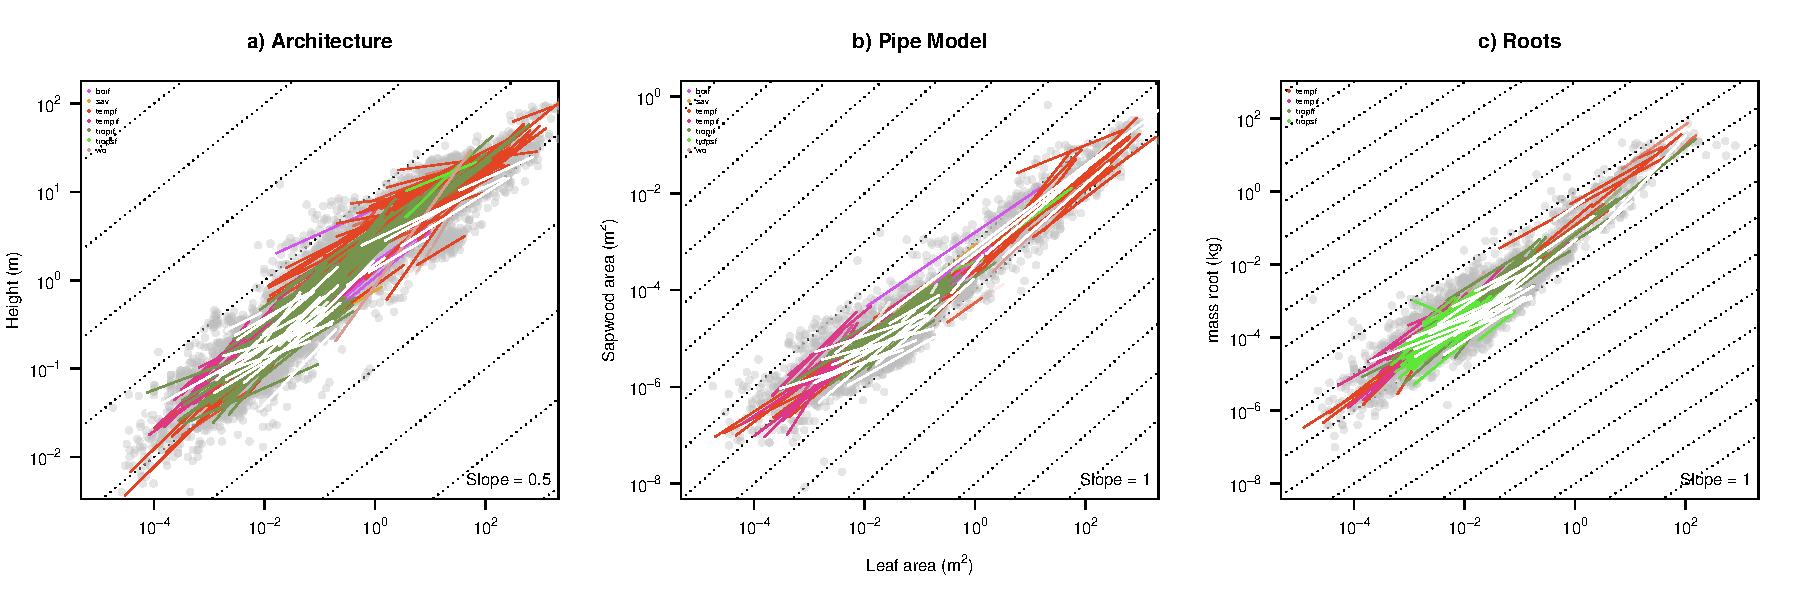
\includegraphics{main/allometry.pdf}
\caption{\textbf{Key assumptions of a functional balance and trait
trade-offs model, evaluated using global dataset.} We used the biomass and
allometry database to evaluate model assumptions about \textbf{a,}
scaling of leaf area with plant height, \textbf{b} Scaling of sapwood
area with leaf area, and \textbf{c} scaling of root mass with leaf area.
Each dot is a single plant. Lines show standardised major axis lines
fitted to data from each site, with intensity of shading adjusted
according to strength of the relationship. Colours indicate vegetation
type. Dashed black lines show values expected under functional-balance
assumption (see Supplementary text for details). \label{fig:assumptions}}
\end{figure}

\newpage

\begin{figure}[ht]
\centering
\includegraphics{main/growth_light_dia.pdf}
\caption{\textbf{Traits moderate the responsiveness of growth to changes
in light environment (diameter growth).} Panels show predicted relationship between
specific trait and diameter growth rate, for a plant of specified
diameter and under a range of shading environments.
\label{fig:growth_light_dia}}
\end{figure}

\begin{figure}[ht]
\centering
\includegraphics{main/growth_light_mass.pdf}
\caption{\textbf{Traits moderate the responsiveness of growth to changes
in light environment (mass growth).} Panels show predicted relationship between
specific trait and diameter growth rate, for a plant of specified
diameter and under a range of shading environments.
\label{fig:growth_light_mass}}
\end{figure}

\newpage

\begin{figure}[ht]
\centering
\includegraphics{main/max_leaf_above.pdf}
\caption{\textbf{The effect of traits on growth changes with size and
light environment.} Traits moderate the responsiveness of growth to changes in light
environmentThis figure needs to show more of key result with respect to to size.
Possibly separate figure. \label{fig:shifts}}
\end{figure}

\newpage

\begin{figure}[ht]
\centering
\includegraphics{main/max_leaf_above.pdf}
\caption{\textbf{Low construction cost leads to shade intolerance,
because of costs of high turnover.} Panels show effect of traits on
maximum amount of shading that can be endured before net production (eqn
\ref{eq:dbdt}) reaches zero. Lines indicate relationship for plants of a
given height. \label{fig:wplcp}}
\end{figure}

\clearpage

\section{Appendices}
\subsection{A - Relationship between traits and relative growth rate} \label{app:traits-RGR}

We start with eqn \ref{eq:dbdt} for mass-based growth. For seedlings, which are
young and mostly leaf, it is reasonable to ignore all turnover terms as
well as the respiration terms for non-leaf tissues. Net production then
becomes a linear function of leaf area and net photosynthesis per leaf
area ($A_\textrm{net} = y(A - r_{\rm l})$), making relative growth
rate a linear function of $\phi$:

\begin{equation}\label{eq:RGR}
\underbrace{\strut\frac{{\rm d}B}{{\rm d}t}\frac{1}{M_{\rm a}}}_\textrm{relative growth in mass}  \approx A_\textrm{net} \times \phi^{-1} \times \frac{M_{\rm l}}{M_{\rm a}}. \end{equation}

Although eqn \ref{eq:RGR} captures patterns of growth in seedlings in
relation to $\phi$\citep{Wright-2000}, this
approximation does not directly link to other traits, or to the
variables that are routinely collected for large trees: namely plant
height ($h$) and stem cross-sectional area ($A_{\rm st}$) or
diameter $D$.

\subsection{B - Effect of traits on height growth} \label{app:traits-RGR}

We want to show how two traits $\phi$ and $\rho$ influence growth rate,
by looking at the effect of
traits on the components of growth rate (eqn \ref{eq:dhdt}. To make
the analysis more tractable, we will assume we are dealing with a plant of
given height where 100\% of available energy is allocated to growth,
i.e. $\frac{{\rm d}M_{\rm a}}{{\rm d}B}=1$. Note also
that by the assumptions of our model and above, traits do not influence
$\frac{{\rm d}H} {{\rm d}A_{\rm l}}$. Thus we have
\begin{equation} \label{eq:G2}
G = \frac{{\rm d}H}{{\rm d}t} = c_1   \left(\frac{{\rm d}A_{\rm l}} {{\rm d}M_{\rm a}}  \frac{ {\rm d}B} {{\rm d}t} \right),
\end{equation}
where $c_1 = \frac{{\rm d}H}{{\rm d}A_{\rm l}}$. Eqn
\ref{eq:G2} is a product of the form $Y(x) = W(x) \times Z(x)$. For,
equations of this type, the derivative $\partial{Y}/\partial{x}$ is
given by $\partial{W}/\partial{x} \, Z + W \, \partial{Z}/\partial{x}$. Thus
the derivative of $G$ with respect to some trait $x$  is given by
\begin{equation} \label{eq:dG}
\frac{\partial G} {\partial x} =
\frac{\partial \left(\frac{{\rm d}A_{\rm l}} {{\rm d}M_{\rm a}}\right)}{\partial x}
 \, \frac{ {\rm d}B} {{\rm d}t}
+ \frac{{\rm d}A_{\rm l}} {{\rm d}M_{\rm a}}
\, \frac{\partial \left( \frac{ {\rm d}B} {{\rm d}t}\right)}{\partial x}.
\end{equation}
If this derivative is positive (negative), there will be a positive (negative) relationship
between traits and growth at the height where it is evaluated.

We can further simplify by expanding the derivative of eqn \ref{eq:daldmt}:
\begin{equation} \label{eq:dA_dx}
\frac{\partial \left(\frac{{\rm d}A_{\rm l}} {{\rm d}M_{\rm a}}\right)}
{\partial x} = -\left(\frac{{\rm d}A_{\rm l}} {{\rm d}M_{\rm a}}\ \right)^2
\, \frac{\partial \left(\frac{{\rm d}M_{\rm a}} {{\rm d}A_{\rm l}}\right)
}{\partial x}.
\end{equation}
Combing eqs. \ref{eq:dG}-\ref{eq:dA_dx}, we have
\begin{equation} \label{eq:dG2}
\frac{\partial G} {\partial x} =
\frac{{\rm d}A_{\rm l}} {{\rm d}M_{\rm a}}
\left(
\frac{\partial \left( \frac{ {\rm d}B} {{\rm d}t}\right)}{\partial x}
- \frac{{\rm d}A_{\rm l}} {{\rm d}M_{\rm a}}
\,  \frac{\partial \left(\frac{{\rm d}M_{\rm a}} {{\rm d}A_{\rm l}}\right)
}{\partial x}
 \, \frac{ {\rm d}B} {{\rm d}t}
\right).
\end{equation}

Since is $\frac{{\rm d}A_{\rm l}} {{\rm d}M_{\rm a}}>0$ always, the sign
of $\frac{\partial G} {\partial x}$ depends on the terms inside the brackets on the
RHS. Rearranging we find that $\frac
{\partial G} {\partial x} < 0$ if
\begin{equation}\label{eq:dg3}
\frac{\partial \left( \frac{ {\rm d}B} {{\rm d}t}\right)}{\partial x}
< \frac{{\rm d}A_{\rm l}} {{\rm d}M_{\rm a}}
\,  \frac{\partial \left(\frac{{\rm d}M_{\rm a}} {{\rm d}A_{\rm l}}\right)
}{\partial x} \, \frac{ {\rm d}B} {{\rm d}t},
\end{equation}
or equivalently
\begin{equation}\label{eq:dg4_orig}
\frac{
\frac{\partial \left( \frac{ {\rm d}B} {{\rm d}t}\right)}{\partial x} }
{\frac{ {\rm d}B} {{\rm d}t}}
<
\frac{ \frac{\partial \left(\frac{{\rm d}M_{\rm a}} {{\rm d}A_{\rm l}}\right)
}{\partial x}}{\frac{{\rm d}M_{\rm a}} {{\rm d}A_{\rm l}}}.
\end{equation}

\subsection{C - Linking traits to whole-plant light compensation point} \label{app:traits-RGR}

\section{Supplementary materials}

\subsection{A -- Full description of the \texttt{FF16} growth model}\label{sec:ff16}

\subsection{B -- Supplementary Figures}\label{sec:SM_figs}

\subsection{C -- Supplementary Tables}\label{sec:SM_tabs}

\footnotesize

\bibliography{references}

\end{document}